\documentclass{beamer}

\usepackage{listings}
\usepackage{tikz}
\usetikzlibrary{arrows,automata,calc,graphs,positioning,shapes,trees}

\def\dblabel{teste=\#\ }
\def\cmd#1{{\tt \char92#1}}
\def\onlytitleframe#1{\author{}\date{}\title{#1}\maketitle}

\title{Administração de Banco de Dados: Arquitetura do PostgreSQL}

\begin{document}
\date{\today}
\frame{\maketitle}

\begin{frame}{Projeto do banco de dados}
  
  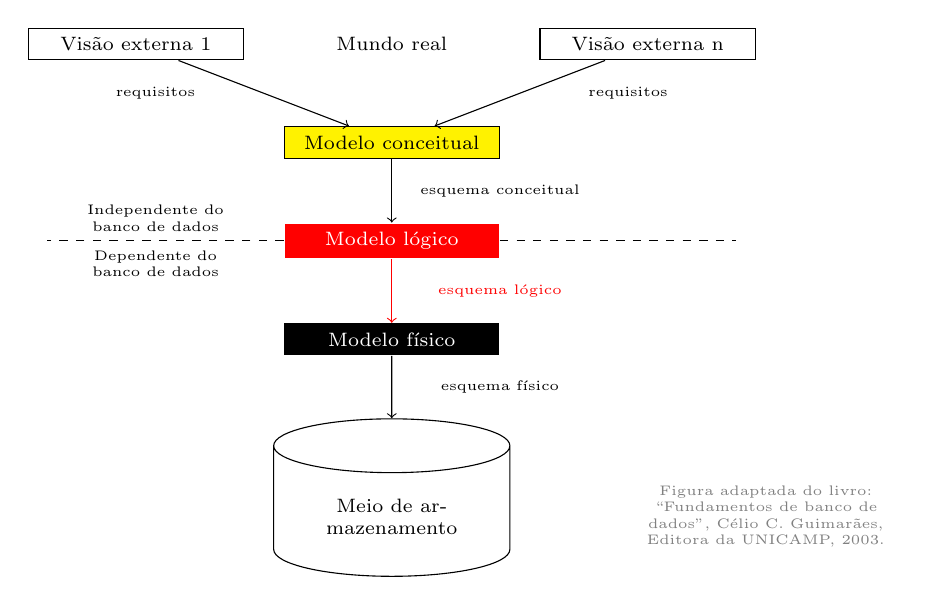
\begin{tikzpicture}[every node/.style={node distance=1.25cm,font=\scriptsize,text width=2.5cm,text centered},
    elem/.style={draw},physical/.style={white,fill=black}]
   
    \node (REAL) {Mundo real};
    \node[elem] (VIEW0) [left of=REAL,xshift=-2cm] {Visão externa 1};
    \node[elem] (VIEWN) [right of=REAL,xshift=2cm] {Visão externa n};
    \node[fill=yellow,draw] (CONCEPTUAL) [below of=REAL] {Modelo conceitual};
    \node[white,fill=red,draw] (LOGICAL) [below of=CONCEPTUAL] {Modelo lógico};
    \node[physical] (PHYSICAL) [below of=LOGICAL] {Modelo físico};
    \node[cylinder,shape border rotate=90,minimum height=2cm,minimum width=3cm,aspect=.25,draw] (DISK) [below of=PHYSICAL,yshift=-1cm] {Meio de armazenamento};

    \draw[dashed] (LOGICAL.west) -- +(-3,0) 
    node[above right,font=\tiny] {Independente do banco de dados} 
    node[below right,font=\tiny] {Dependente do banco de dados};
    \draw[dashed] (LOGICAL.east) -- +(3,0);

    \path[->,draw] (VIEW0) -- node[font=\tiny,left] {requisitos} (CONCEPTUAL);
    \path[->,draw] (VIEWN) -- node[font=\tiny,right] {requisitos} (CONCEPTUAL);
    \path[->,draw] (CONCEPTUAL) -- node[right,font=\tiny] {esquema conceitual} (LOGICAL);
    \path[red,->,draw] (LOGICAL) -- node[right,red,font=\tiny] {esquema lógico} (PHYSICAL);
    \path[->,draw] (PHYSICAL) -- node[right,font=\tiny] {esquema físico} (DISK);

    \node[gray,text width=3.5cm,text centered,font=\tiny] [right of=DISK,xshift=3.5cm] {Figura adaptada do livro: ``Fundamentos de banco de dados'', Célio C. Guimarães, Editora da UNICAMP, 2003.};
  \end{tikzpicture}

\end{frame}

\begin{frame}{Arquitetura de comunicação}{Cliente/Servidor}
  
\begin{center}
  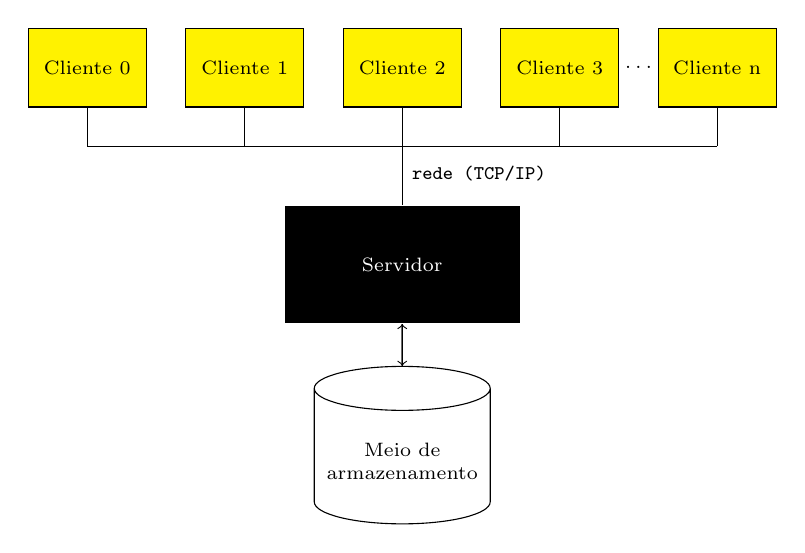
\begin{tikzpicture}[every node/.style={font=\scriptsize},
    client/.style={minimum width=1.5cm,minimum height=1cm,fill=yellow,draw}]

    
    \node[white,fill=black,minimum width=3cm,minimum height=1.5cm,draw] (SERVER) {Servidor};
    \node[cylinder,shape border rotate=90,text width=2cm,text centered,minimum height=2cm,minimum width=1.5cm,aspect=.25,draw] (DISK) [below of=SERVER,yshift=-1.5cm] {Meio de armazenamento};

    \foreach \x/\l in {-4/0,-2/1,0/2,2/3,4/n} {
      \node[client] (CLIENT\l) [above of=SERVER,xshift=\x cm,yshift=1.5cm] {Cliente \l};
      \path[draw] (CLIENT\l) -- +(0,-1);
    }
    \path[draw] (CLIENT0)+(0,-1) -- +(8,-1);
    \path[draw] (CLIENT2) -- node[below right] {\tt rede (TCP/IP)} (SERVER);
    
    \node [right of=CLIENT3] {$\ldots$};

    \path[->,draw] (SERVER) -> (DISK);
    \path[->,draw] (DISK) -> (SERVER) ;
  \end{tikzpicture}
\end{center}

\end{frame}

\begin{frame}{Arquitetura do sistema PostgreSQL}
  
  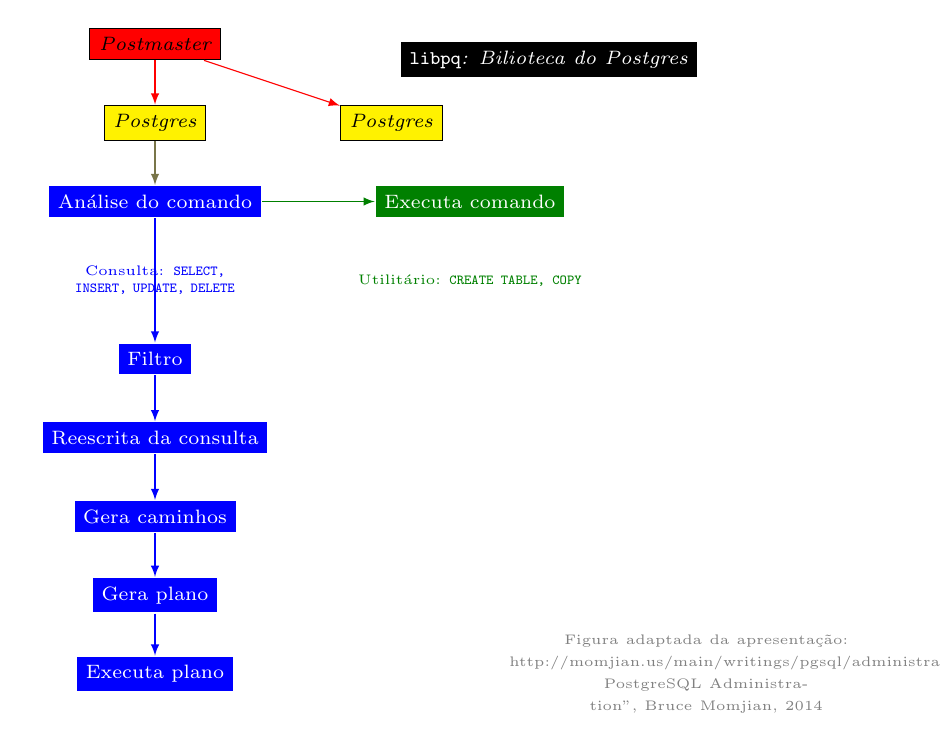
\begin{tikzpicture}
    [every node/.style={font=\scriptsize},
    elem/.style={draw},
    postmaster/.style={elem,fill=red},
    libpq/.style={elem,white,fill=black},
    postgres/.style={elem,fill=yellow},
    every path/.style={->,>=latex,draw},
    query/.style={elem,white,fill=blue},
    utility/.style={elem,white,fill=green!50!black}]
    
    \node[postmaster] (POSTMASTER) {\it Postmaster};
    \node[libpq] (LIBPQ) [right of=POSTMASTER,xshift=4cm,yshift=-.2cm] {\it {\tt libpq}: Bilioteca do Postgres};
    \node[postgres] (POSTGRES0) [below of=POSTMASTER] {\it Postgres};
    \node[postgres] (POSTGRES1) [right of=POSTGRES0, xshift=2cm] {\it Postgres};
    \node[query] (PARSE) [below of=POSTGRES0] {Análise do comando};
    \node[text width=3cm, text centered,blue,font=\tiny,fill=white] (QUERYCMD) [below of=PARSE] {Consulta: \tt SELECT, INSERT, UPDATE, DELETE};
    \node[query] (FILTER) [below of=QUERYCMD] {Filtro}; % traffic cop
    \node[query] (REWRITE) [below of=FILTER] {Reescrita da consulta};
    \node[query] (PATHS) [below of=REWRITE] {Gera caminhos};
    \node[query] (PLAN) [below of=PATHS] {Gera plano};
    \node[query] (EXEC) [below of=PLAN] {Executa plano};
    \node[utility] (UTILITY) [right of=PARSE,xshift=3cm] {Executa comando};
    \node[font=\tiny,green!50!black] (UTILCMD) [below of=UTILITY] {Utilitário: \tt CREATE TABLE, COPY};

    \path[red] (POSTMASTER) -- (POSTGRES0);
    \path[red] (POSTMASTER) -- (POSTGRES1);
    \path[yellow!40!black] (POSTGRES0) -- (PARSE); 
    \path[blue] (PARSE) -- (FILTER);
    \path[blue] (FILTER) -- (REWRITE);
    \path[blue] (REWRITE) -- (PATHS); 
    \path[blue] (PATHS) -- (PLAN);
    \path[blue] (PLAN) -- (EXEC);
    \path[green!50!black] (PARSE.east) -- (UTILITY);
   
    \node [gray,right of=EXEC,xshift=6cm,text width=5cm,text centered] {\tiny Figura adaptada da apresentação:
    \href{http://momjian.us/main/writings/pgsql/administration.pdf}{``Mastering
      PostgreSQL Administration'', Bruce Momjian, 2014}};
  \end{tikzpicture}

\end{frame}

%% ??? if the database occupies TB how is it stored in shared memory ???
%% ??? how table spans along the file nodes of shared memory ???

\lecture{Estrutura de memória}{mem}

\onlytitleframe{\insertlecture}

\begin{frame}{\insertlecture}

  O sistema Postgres utiliza {\bf memória compartilhada} para
  armazenamento de dados e comunicação entre os processos. A memória
  compartilhada é dividida em {\bf páginas} com as seguintes
  características:
  
  \begin{itemize}
  \item Tamanho fixo de páginas: {\bf 8KB};
  \item Mapa de espaço livre (FSM--{\it free space map\/});
  \item Mapa de visibilidade (VM--{\it visibility map\/}): tuplas visíveis a todas as transações ativas.
  \end{itemize}
  
\end{frame}


\begin{frame}{Banco de dados}{Sistemas de arquivos}
  
  \begin{tikzpicture}[every node/.style={minimum height=.5cm,font=\tiny},
    item/.style={fill=yellow,anchor=east,draw},
    tuple/.style={fill=gray!30,anchor=west,draw}]
  
    \node at (0,5cm) {\tt \$POSTGRES\_DIRECTORY/data/base/};

    \node[] at (4cm,6cm) {\tt base/}
    [edge from parent fork down]
    child {node {{\tt 1/} (template1)}}
    child {node {{\tt 16384/} (test)}
    };
  \end{tikzpicture}    

\end{frame}

\begin{frame}{Tabelas}{Sistemas de arquivos}
  Estrutura de páginas

  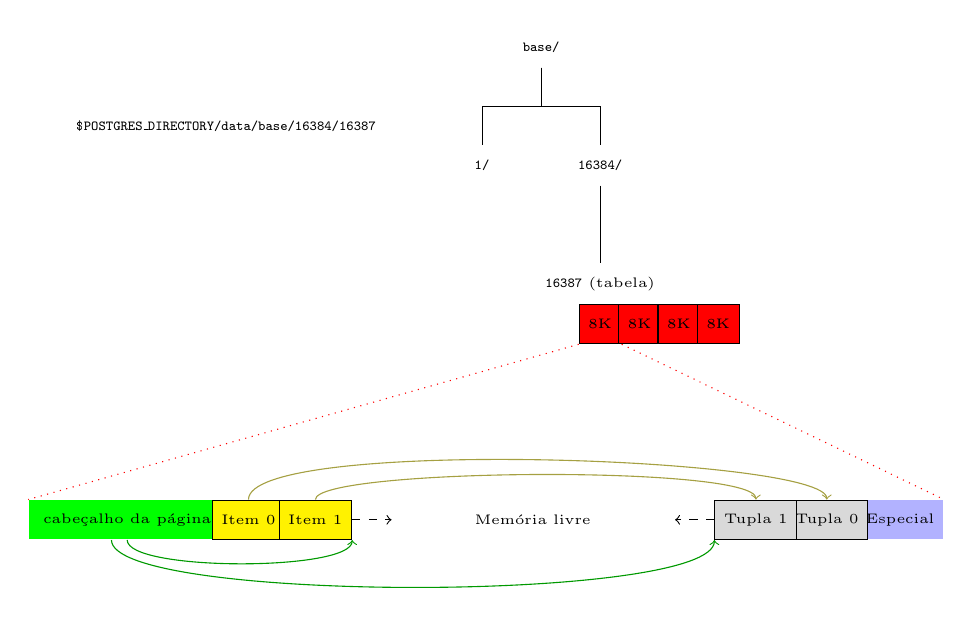
\begin{tikzpicture}[every node/.style={minimum height=.5cm,font=\tiny},
    item/.style={fill=yellow,anchor=east,draw},
    tuple/.style={fill=gray!30,anchor=west,draw}]
  
    \node at (0,5cm) {\tt \$POSTGRES\_DIRECTORY/data/base/16384/16387};

    \node[] at (4cm,6cm) {\tt base/}
    [edge from parent fork down]
    child {node {\tt 1/}}
    child {node {\tt 16384/}
      child[] {node (LEAF) {{\tt 16387} (tabela)}}
    };
    
    \foreach \i in {0,1,2,3} \node[fill=red,draw] (PAGE\i) [below=of LEAF,xshift=\i*.5 cm,yshift=1cm] {8K};

    \node[anchor=east,fill=green,minimum width=2.5cm] (HEADER) at (0,0) {cabeçalho da página};
    \node[item] (ITEM0) at (.75cm,0) {Item 0};
    \node[item] (ITEM1) at (1.6cm,0) {Item 1};
    \path[->,dashed,draw] (ITEM1.east) -- +(.5cm,0);

    \node[minimum width=4.6cm,anchor=east] at (6.2cm,0) {\rm Memória livre};

    \node[anchor=west,fill=blue!30,minimum width=1cm] (SPECIAL) at (8cm,0) {Especial};
    \node[tuple] (TUPLE0) at (7.1cm,0) {Tupla 0};
    \node[tuple] (TUPLE1) at (6.2cm,0) {Tupla 1};
    \path[->,dashed,draw] (TUPLE1.west) -- +(-.5cm,0);

    \draw [yellow!60!black,->] (ITEM0.north) .. controls +(up:8mm) and +(up:8mm) .. (TUPLE0);
    \draw [yellow!60!black,->] (ITEM1.north) .. controls +(up:4mm) and +(up:7mm) .. (TUPLE1);

    \draw [green!60!black,->] (HEADER.south) .. controls +(down:4mm) and +(down:4mm) .. (ITEM1.south east);
    \draw [green!60!black,->] (HEADER.south)+(-.2,0) .. controls +(down:8mm) and +(down:8mm) .. (TUPLE1.south west);

    \path[red,dotted,draw] (PAGE0.south west) -- (HEADER.north west);
    \path[red,dotted,draw] (PAGE0.south east) -- (SPECIAL.north east);

  \end{tikzpicture}

\end{frame}

\begin{frame}{Tupla}{Sistema de arquivos}
  
  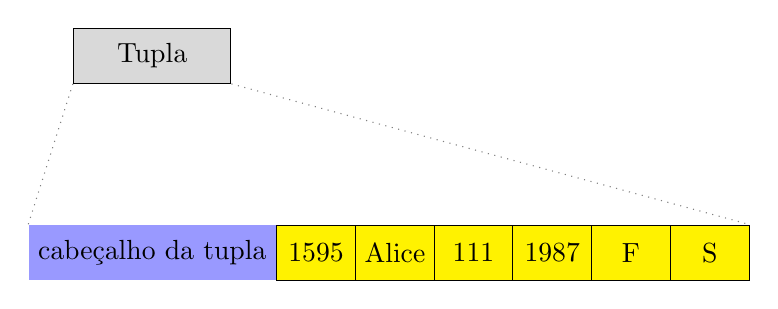
\begin{tikzpicture}[every node/.style={minimum height=.7cm},
    value/.style={fill=yellow,minimum width=1cm,draw}]
    \node[fill=gray!30,minimum width=2cm,draw] (TUPLE) {Tupla};

    \node[fill=blue!40] (HEADER) [below of=TUPLE,yshift=-1.5cm] {cabeçalho da tupla};

    \foreach \i/\v in {0/1595,1/Alice,2/111, 3/1987, 4/F, 5/S} {
      \node<1>[value] (VALUE\i) [right=of HEADER,xshift=\i cm-1cm] {valor};
      \node<2>[value] (VALUE\i) [right=of HEADER,xshift=\i cm-1cm] {\v};
  }
  \path[gray,dotted,draw] (TUPLE.south west) -- (HEADER.north west);
    \path[gray,dotted,draw] (TUPLE.south east) -- (VALUE5.north east);

  \end{tikzpicture}
  
\end{frame}

\begin{frame}{Referências}
  
  \begin{itemize}
  \item Bruce Momjian.
    \href{https://momjian.us/main/writings/pgsql/inside_shmem.pdf}{``Inside PostgreSQL Shared Memory''}, 2015.
  \item Bruce Momjian. \href{http://momjian.us/main/writings/pgsql/internalpics.pdf}{``'PostgreSQL Internals Through Pictures''}, 2012.
  \item The PostgreSQL Global Development
    Group. \href{http://www.postgresql.org/docs/9.4/interactive/index.html}{``PostgreSQL 9.4.4 Documentation''}, 2015.
  \end{itemize}
\end{frame}

\begin{frame}[fragile]{GRANT}

  \begin{lstlisting}
 test=> CREATE VIEW customer_ohio AS                 
        test-> SELECT * 
        test-> FROM customer 
        test-> WHERE state = 'OH'; 
        CREATE 18908 1 
        test=> 
        test=> -- let sanders see only Ohio customers 
        test=> GRANT SELECT ON customer_ohio TO sanders; 
        CHANGE
      \end{lstlisting}
    \end{frame}

    \end{document}

